
\section{Generating realistic data} %0.5-1
\thispagestyle{plain}
We as humans have been born with the blessing of intelligence. We use this intelligence to create things of indescribable creativity and complexity and it is these things that give a deeper meaning to large parts of human life. All the greater is the drive to understand this creative process and to reproduce it artificially. And it is this drive that gave rise to a completely new branch of research in computer sciences, which finally led to the concept of \textit{Generative Modeling}.

\thispagestyle{plain}
Generative Modeling is an umbrella term describing artificial approaches to generate realistic data. The current state-of-the-art approaches are dominated by so called \textit{Deep Neural Networks}, complex artificial constructs which are partially inspired by the human brain. These networks are implemented as a computer program, using modern machine learning libraries such as \textit{PyTorch} or \textit{Tensorflow}.

\thispagestyle{plain}
In the last years generative modeling has seen an \textbf{immense} progress in generating the most diverse types of data. Some results have even reached such a quality that they can hardly be distinguished from realistic data for the human eye. Some fields of generative modeling on which outstanding results have been achieved include image generation, video generation and audio and speech generation. In addition to the general push for better generation models, some models are already indispensable for various application purposes such as image processing, anomaly detection in medical context and generation of new data for scientific uses, e.g. the artificial generation of promising molecular candidates for the development of new effective drugs \cite{molgrad}.
\thispagestyle{plain}
%%%%%%%%%%%%%%%%%%%%%%%%%%%%%%%%%%%%%%%%%%%%%%%%%%%%%%%%%%%%%%%%%%%%%%%%%%%%%%%%%%%%%%%%%%%%
\section{Score-Based Generative Models - The new contenders to GANs?} 
\thispagestyle{plain}
Score Based Generative Models (SGMs) were recently proposed by Yang Song and Stefano Ermon \cite{score_1} in late 2020. As a generative model SGMs can be used to generate all kinds of data such as images, audio and graphs and they are capable of performing a variety of special tasks such as inpainting, colorization and image-to-image translation. As shown in outstanding results from recent work \cite{score_3} they are absolutely capable to keep up with state-of-the-art generative models such as Generative Adversarial Networks (GANs) \cite{gan_original} and Variational Autoencoders (VAEs) \cite{vae_original}. Therefore SGMs have gained great attention in the scientific community and are already considered by some to be the "new contenders to GANs".

\thispagestyle{plain}
Score-Based Generative Models work by estimating the score of a given data distribution via score matching \cite{score_matching_original}. Because the score estimating technique is unstable or ill-defined for a real data distribution the initial images are perturbed by Gaussian noise. Starting from random noise, SGMs are able to generate completely new data. To put it in the words of the inventors: "Creating noise from data is easy; creating data from noise is generative modeling [with SGMs]".

\thispagestyle{plain}
%
\begin{figure}[]
    \centering
    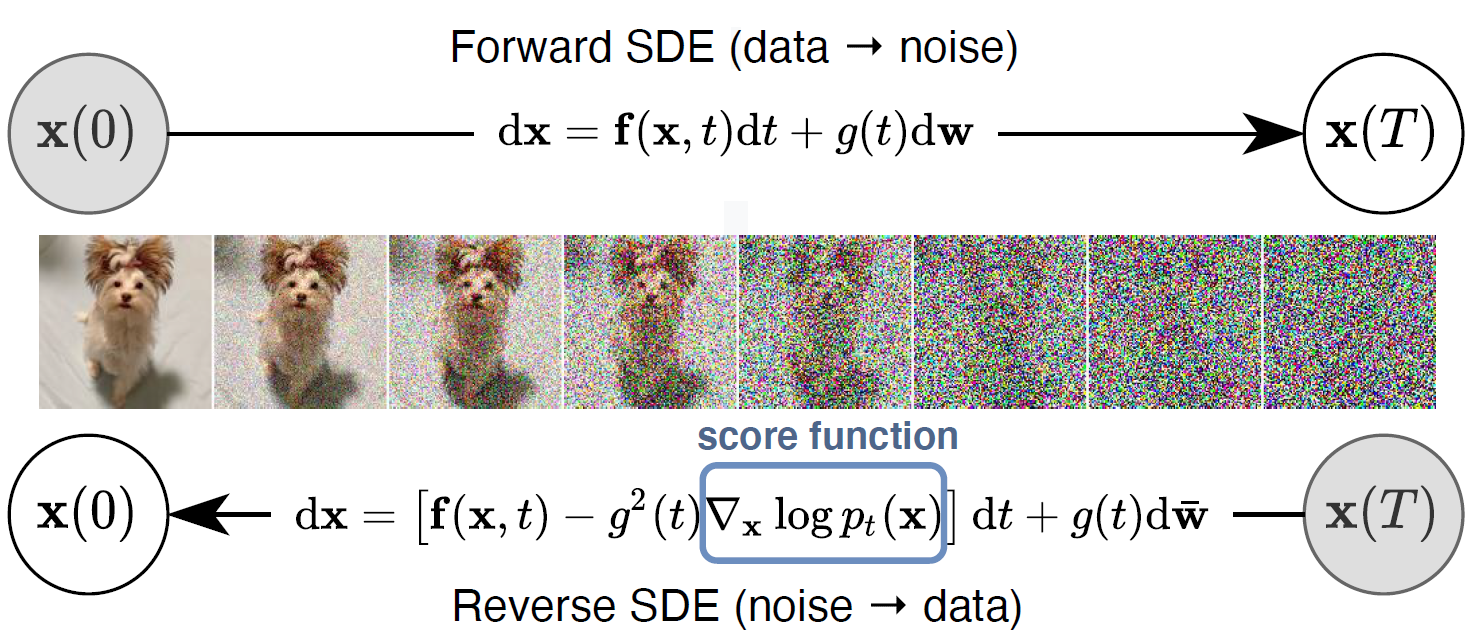
\includegraphics[width=0.8\textwidth]{Chapters/figures/sgm.PNG}
    \caption{The idea of SGMs: First the data distribution is perturbed via a diffusion process governed by a SDE. The scores of the noise distributions are learned by the score-model and are then used to solve a reverse SDE to generate new data from noise.}
\end{figure}
%

\thispagestyle{plain}
SGMs have several advantages to other popular models. They do not rely on adversarial training, which is often unstable, they do not need a special architecture in order to be tractable, they do not need sampling during training and they can be used for different tasks such as inpainting, class-conditional generation and colorization without the need to retrain the model. Although SGMs are very slow in sampling, they have the advantage that the sampling process is completely decoupled from the training process, allowing any combination of sampling techniques and model architectures for optimal sampling. All in all these properties, together with the high quality of the recent results, make SGMs a promising new model for generative modeling.
%%%%%%%%%%%%%%%%%%%%%%%%%%%%%%%%%%%%%%%%%%%%%%%%%%%%%%%%%%%%%%%%%%%%%%%%%%%%%%%%%%%%%%%%%%%%%%%
\section{Semantic Segmentation and Semantic Synthesis} 
\thispagestyle{plain}
%
\begin{figure}[h!]
    \centering
    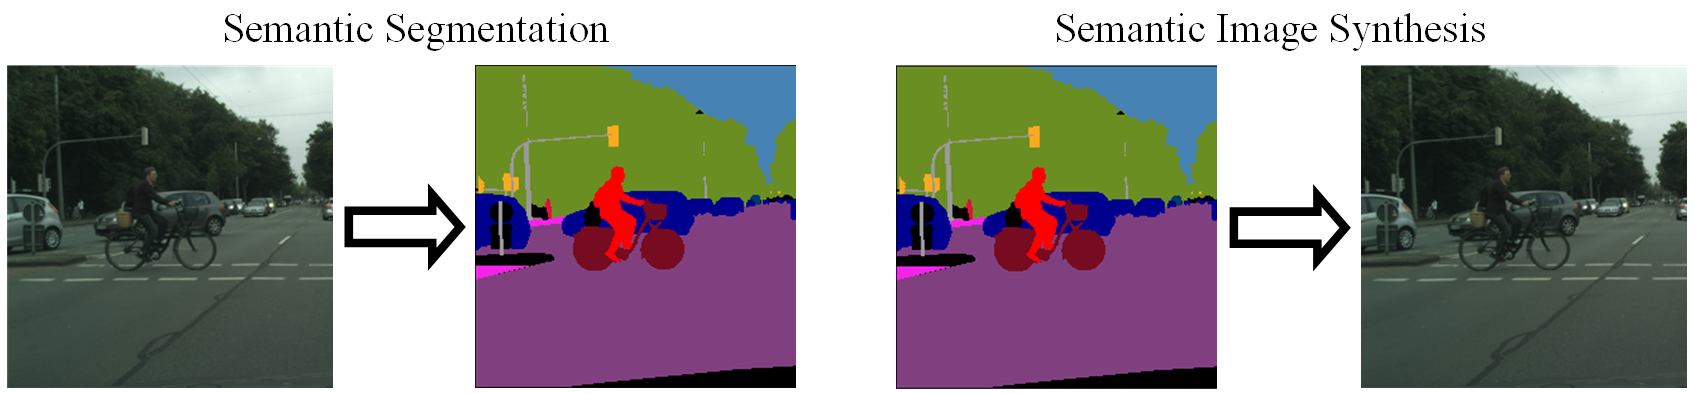
\includegraphics[width=1\textwidth]{Chapters/figures/sem_seg_vs_sem_synth.PNG}
\end{figure}
%
Two large fields in image based machine learning are semantic segmentation and semantic image synthesis. In semantic segmentation so called semantic segmentation networks have the task of a pixel-wise classification of images. In semantic image synthesis – unlike unconditioned image generation \cite{score_3} – images are generated based one a given semantic label map.

In this thesis we show that Score-Based Generative Models, with the help of semantic segmentation networks, are capable of synthesizing realistic looking images based on semantic label maps for various resolutions up to $1024\times512$ and datasets such as Cityscapes \cite{cityscapes}, ADE20K \cite{ade20k} and landscape images scraped from flickr. We show that the synthesized images for some categories can keep up with or even surpass state of the art generative models such as CRN \cite{crn}, pix2pixHD \cite{pix2pixHD}, and SPADE \cite{spade}, although there is still room for further improvement. We therefore show how the current technique could be optimized in future work to yield even better results. 

The implementation for this work is done with PyTorch and the code is publicly available on GitHub at the following links: 
\begin{itemize}
    \item https://github.com/TimK1998/SemanticSynthesisForScoreBasedModels
    \item https://github.com/TimK1998/SemanticSegmentation
\end{itemize}
